%
% Hinweis:
%
% Die Tabellenanordnung, etc muss noch überprüft werden.
% Teilweise sind Figures auf der falschen Seite, trotz [h!]
%

\chapter{Topic 9 -- Testing Non-Functional Requirements with Risk Analysis}

\section{Introduction}

In contrast to \glspl{FR} that describe the program's functionality, i.e. how it processes data and user input, \glspl{NFR} describe constraints that the program must adhere to~\cite{SWEBOK}.
Parts of \glspl{NFR} are performance and security requirements which can directly affect the end-user but also maintainability requirements which are more important to development teams.
While there are lot of resources about testing \glspl{FR} in the form of unit-, integration- and end-to-end-tests, no common testing framework or guidance for testing \glspl{NFR} exists.

For this reason, we look into two approaches \cite{ZouPavlovski2008} and \cite{Lagerstedt2014}.
While \cite{ZouPavlovski2008} was given in advance by the advisors of the seminar, \cite{Lagerstedt2014} was found through a literature search, which is described in \autoref{sec:9_literature}.
Each approach will be described and applied to an example in the form of movie management software in the respective sections \ref{sec:9_approach_1} and \ref{sec:9_approach_2}. 

Both approaches are compared in \autoref{sec:9_comparison} by using a synthesis matrix. We will look at which \glspl{NFR} are covered and how they are tested.
The results of this chapter will be summarized and concluded in \autoref{sec:9_conclusion}.

Please refer to the glossary for the following terms used throughout this chapter:
test case, use case, NFR.



%%%%%%%%%%%%%%%%%%%%%%%%%%%%%%%%%%%%%%%%%%%%%%%%%%%%%%%%%%%%%%%%%%%%%%%%%%%%%%
%%%%%%%%%%%%%%%%%%%%%%%%%%%%%%%%%%%%%%%%%%%%%%%%%%%%%%%%%%%%%%%%%%%%%%%%%%%%%%

\section{Literature Search} \label{sec:9_literature}

The starting point for the literature search was the paper given to us~\cite{ZouPavlovski2008}.
Based on this paper, we formulated the central research question: 

\hspace*{0.5cm}\enquote{\textit{Which approaches for testing non-functional requirements systematically\newline \hspace*{0.7cm}with risk analysis exist?}}.

We focused on finding articles that covered the three most important keywords and phrases for the topic: \textit{testing}, \textit{non-functional requirements} and \textit{risk analysis}.
A quick search using these three phrases resulted in IEEE Xplore having the most promising results, whereas ACM\footnote{\url{https://dl.acm.org/}} only showed a few.
Because the given article \cite{ZouPavlovski2008} can also be found on IEEE~Xplore\footnote{\url{https://ieeexplore.ieee.org/Xplore/home.jsp}}, we focused our search onto that site but still looked at ACM.

To be able to evaluate the relevance of papers found during the literature search, we defined three relevance criteria:

\begin{enumerate}
	\item Does the article cover non-functional requirements? They must not only  be mentioned as a side note next to functional requirements.
	\item Does the article combine risk analysis with tests?
	\item Does the article cover \textit{testing} of non-functional requirements?
\end{enumerate}

Even though these relevance criteria basically only cover the research question, they filter out most non-relevant papers as we will see later on.

% https://ieeexplore.ieee.org/document/4578345
The search was carried out by using forward and backward snowballing as well as by using search terms with combinatorial modifiers.
Only two papers reference \cite{ZouPavlovski2008} according to its IEEE~Xplore site, both of which cover functional but not non-functional requirements.
The paper itself references 23 papers.
Of those papers, only few covered the first criterion and none covered the third criterion.
\cite{ZouPavlovski2008} itself does not cover risk analysis as a main research topic but only covers it in a side note (see \autoref{sec:9_approach_1}).
This is why search-term based search was performed using the key terms: non-functional requirements, testing and risk analysis.

\autoref{tbl:search_topic_9_andre} lists an excerpt of the term-based search.
Listed are only those searches that returned promising results or highlight issues I encountered during the search.
It can be seen that, if all keywords are combined using the \texttt{AND} operator with the default restrictions, no relevant results were returned.
After a feedback from one advisor, the search was changed so that \enquote{non-functional requirements} and \enquote{testing} were expected in the paper's abstract, but \enquote{risk analysis} was searched for in \textit{all} metadata including the full text.
It turned out that no papers were found which mentioned risk analysis as well as the other two keywords in their abstract.

We also discovered that the spelling of the term \enquote{non-functional} had a huge impact on the results returned by IEEE~Xplore.

\begin{small}
	\centering
	\begin{longtable}[h]{p{0.08\textwidth}|c|p{0.58\textwidth}|p{0.12\textwidth}}
		\caption{Term based search results}
		\label{tbl:search_topic_9_andre}
		\setlength{\tabcolsep}{1em}\\    %%%%<===
		\toprule
		\textbf{Source} & \textbf{Date} & \textbf{Search query and restrictions} & \textbf{\#Results (relevant)} \\
		
		\midrule
		IEEE Xplore & 2020-11-11 & \texttt{"{}non-functional requirements"{} AND testing AND "{}risk analysis"{}} & 3 (0) \\
		
		\midrule
		IEEE Xplore & 2020-11-11 & \texttt{non-functional requirements AND testing AND risk analysis} & 12 (0) \\
		
		\midrule
		IEEE Xplore & 2020-11-11 & \texttt{risk AND "non-functional" and test} & 23 (2) \\
		
		\midrule
		IEEE Xplore & 2020-11-29 & \texttt{(("{}Abstract"{}:nonfunctional requirements) AND "{}Abstract"{}:Test) AND "Full Text \& Metadata":"{}risk analysis"{})} & 2 (1) \\
		
		\midrule
		IEEE Xplore & 2020-11-29 & \texttt{(("{}Abstract"{}:non-functional requirements) AND "{}Abstract"{}:Test) AND "Full Text \& Metadata":"{}risk analysis"{})} & 3 (0) \\

		\midrule
		ACM & 2020-11-29 & \texttt{[Abstract: "{}risk"{}] AND [Abstract: test*] AND [Abstract: "{}non functional"{}]} & 4 (1) \\
		
		\midrule
		ACM & 2020-11-29 & \texttt{[Abstract: test] AND [Abstract: "{}non functional"{}] AND [[Full Text: "{}risk analysis"{}] OR [Full Text: "{}risk"{}]]} & 20 (1) \\
		\bottomrule
	\end{longtable}
\end{small}

After this initial search, the resulting papers were evaluated and one paper was chosen. The papers to chose from included:

\begin{itemize}
	\item \enquote{Scenario-Based Assessment of non-functional Requirements } \cite{Andre_Search_1}
	\item \enquote{Alignment of requirements specification and testing: A systematic mapping study} \cite{Andre_Search_2}
	\item \enquote{Using Automated Tests for Communicating and Verifying Non-functional Requirements} \cite{Lagerstedt2014}
\end{itemize}


\textit{Scenario-Based Assessment of non-functional Requirements} covers all three criteria we defined at the start of our search. However, it limits itself to complex socio-technical systems and only looks at one non-functional requirement, which is the system's performance.  It limits itself to the evaluation of the reliability of certain aspects of software which interacts with humans to calculate the risk of human errors occurring.
This is done by implementing scenarios--hence the title \enquote{scenario-based assessment}. The testing aspect of this paper is limited to human-interactions whose risks are evaluated. If scenarios fail this risk assessment, then so will the test.

\textit{Alignment of requirements specification and testing: A systematic mapping study} is about papers that cover non-functional requirements. It is a study about such papers and lists approaches that are used to test \glspl{NFR}. Some of which are mentioned in other chapters of this paper. However, none cover risk analysis. The paper itself does not give much insight into testing non-functional requirements itself.

The chosen article which we will further evaluate in the following sections is \textit{Using Automated Tests for Communicating and Verifying Non-functional Requirements}. It covers the non-functional requirement \enquote{maintainability} and how it can be tested. It further explains it by using practical examples.
However, the chosen paper does not cover risk-analysis. Since no paper could be found that covers all criteria, we were advised to focus on the testing of non-functional requirements and leave out risk-analysis.


%%%%%%%%%%%%%%%%%%%%%%%%%%%%%%%%%%%%%%%%%%%%%%%%%%%%%%%%%%%%%%%%%%%%%%%%%%%%%%
%%%%%%%%%%%%%%%%%%%%%%%%%%%%%%%%%%%%%%%%%%%%%%%%%%%%%%%%%%%%%%%%%%%%%%%%%%%%%%


\section{Approach 1} \label{sec:9_approach_1}


\subsection{Description of Approach 1}

In their paper \enquote{Control Cases during the Software Development Life-Cycle}~\cite{ZouPavlovski2008}, J. Zou und C. J. Pavlovski based their work on so called  \enquote{control cases} and \enquote{operating conditions} as tools for modeling and controlling \glspl{NFR}.

\enquote{Control cases} are used as a format to communicate and discuss \glspl{NFR} between management, requirement engineers, developers, and system users and to define qualitative attributes of the system.

Their work focuses on determining and revealing problems early on, for example bad performance or security risks.
The classic software development life cycle often focuses on these topics too late or not at all.
However, control cases require \glspl{NFR} to be defined first.
To define them, the paper starts by introducing operating conditions.
Operating conditions model constraints that apply to the system or a specific use case. These constraints are then used to model \glspl{NFR}, hence the operating condition can be seen as a high level view on \glspl{NFR}.
Defining such constraints that apply to a certain use case is left to the reader or rather is mentioned as a step of the business process modeling.

Operating conditions can belong to one or more use cases and are not unique to a specific one. Conditions such as \enquote{Transaction Volume Condition: $>$400 concurrent users} can be applied to different use cases~\cite{ZouPavlovski2008} and model exactly that: a condition under which the use case operates.

Control cases--as the name suggests--control the operating conditions and can be used to ensure that they are complied to.
This makes it possible to mitigate business risks which may affect the business if the operating condition and its constraints are violated.
Their paper visualizes the connection between these artifacts using an \glspl{UML} diagram, which can be seen in \autoref{fig:topic_9_appraoch_1_use_case} below.

\begin{figure}[htbp]
	\centering
	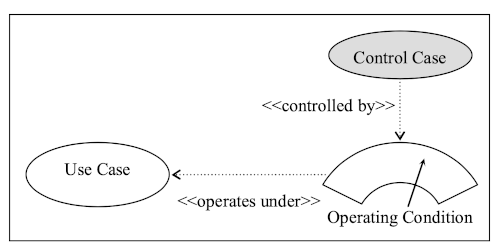
\includegraphics[width=0.5\textwidth]{../images/topic_9_approach_1_1.png}
	\caption{Association in Use Cases Modelling~\cite{ZouPavlovski2008}}
	\label{fig:topic_9_appraoch_1_use_case}
\end{figure}

The paper creates such a control case by introducing a fictional example of a traveling agent.
All of the previously mentioned artifacts are created during the \enquote{Business Process Modeling} and are refined throughout the software development life cycle.
This means that operating conditions and control cases are defined together with use cases and can be incorporated together in a use case model.
The paper does this for their fictional example which can be seen in \autoref{fig:topic_9_appraoch_1_2}. 

\begin{figure}[h!]
	\centering
	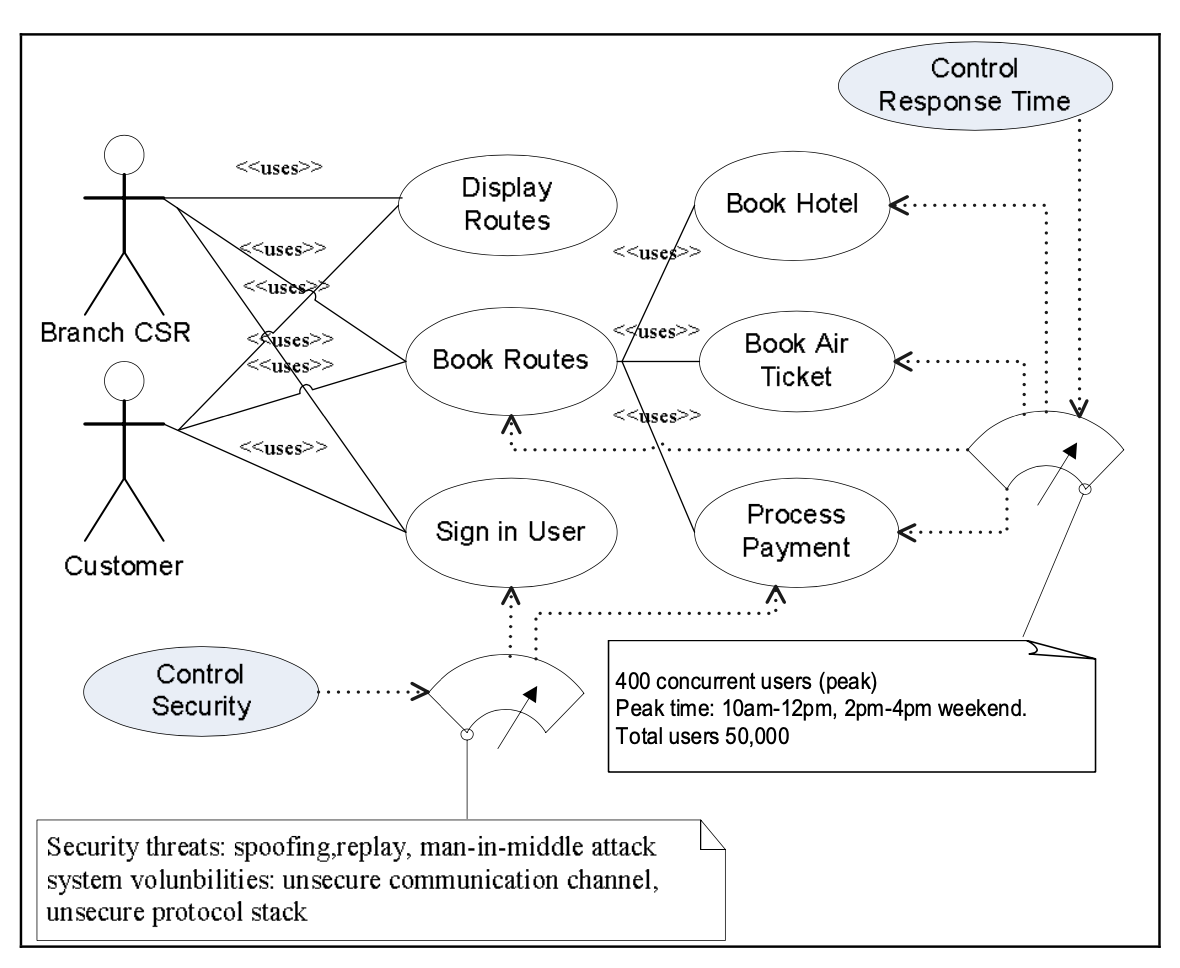
\includegraphics[width=0.7\textwidth]{../images/topic_9_approach_1_2.png}
	\caption{Use Case Model with Control Cases~\cite{ZouPavlovski2008}}
	\label{fig:topic_9_appraoch_1_2}
\end{figure}

In this graphic, control cases are visualized as shaded ellipses and operating conditions as speedometers, though unspecified by the paper. 
This graphic also emphasizes that operating conditions are not bound to one specific use case but can be applied to different ones.
And the control case is specific to one operating condition.


The reader is guided through all steps of the software development life cycle, so that a control case can be defined which is then used as the basis for a test case. Because the control case is associated to an operating condition, the test case is associated to it transitively as well.
The test case exists to verify that the controls put in place to manage the operating condition are effective.

The paper does not give a detailed instruction how to model test cases. It only instructs testers to simulate the operating condition, for example by creating a huge work load on the server.
With this simulation relevant metrics can be extracted that are used to verify the test case.



\subsection{Application of Approach 1}

J. Zou und C. J. Pavlovski focus on creating control cases. This is done for the movie manager example.

We first define one goal of our software:
it must contain a movie list view that has smooth scrolling and can handle a large amount of movies.
This also defines a constraint and therefore our operating condition: we must operate a smooth list view.
If this cannot be accomplished an associated risk may affect the business. The control case bundles all of this in a matrix which is defined as in \autoref{tbl:topic_9_approach_1} on \autopageref{tbl:topic_9_approach_1}.

Based on this control case, developers can start to implement the software. During
testing stage, functional requirements can be tested by basing them on use cases. Non-functional requirements, on the other hand, can be tested by creating tests from control cases.
The tester needs to simulate the operating condition.
In our example above, that would mean to simulate the scrolling condition by creating a huge list of movies.
The steps that must be executed for the test are combined into a test case , such as \autoref{tbl:topic_9_test_case} on \autopageref{tbl:topic_9_test_case}.

By determining the operating condition that is associated to a use case, we were able to create a control case that reflects the \glspl{NFR}.
Based on the operating condition, we then created a test case that checks if the controls put in place by the control cases are enough to mitigate the business risk.
Following this pattern, tests for non-functional requirements can be created systematically step by step.

\clearpage

\begin{table}[h!]
	\centering
	\caption{Control Case for Approach 1 of Topic 9}
	\label{tbl:topic_9_approach_1}
	\begin{tabular}{|p{0.95\textwidth}|}\hline
		\textbf{Control Case}: Performance of the movie list view \\ 
		\hline
		\textbf{Control Case ID}: CC-001 \\
		\hline
		\textbf{Operating Condition}: Scrolling Speed Condition \\
		\hline
		\textbf{Description}: The control case describes the \enquote{smoothness} while scrolling through the movie list view. Scrolling must be smooth. If it is not then users may assume bad performance. \\
		\hline
		\textbf{NFR Category}: Performance and Capacity\\
		\hline
		\textbf{Associated Use Cases}: Show movies in list view \\
		\hline
		\textbf{Technical Constraints}: GUI Framework, Operating System (e.g. 32bit system only allows addressing of 4GB main memory) \\
		\hline
		\textbf{Vulnerability}: \newline Unknown number of movies. Users may only have a few or thousands of movies.
		Analyzing movies (or doing other work) must not lead to the movie list view being unresponsive. Having a lot of movies must not make the program run out of memory. \\
		\hline
		\textbf{Threat Source}: None (local software used by one user) \\
		\hline
		\textbf{Operating Condition}: There may be tens of thousands of movies. Assuming that each movie object has a size of 600kB (only meta data and a small thumbnail), loading 20,000 movies would lead up to 12GB of memory usage\tablefootnote{From personal experience by maintaining a media manager. Users regularly report more than 10,000 movies in their database.}. All movies must be represented in a list view.\\
		\hline
		\textbf{Business Risk}:\newline If scrolling is not smooth, the user may switch to other software or leave a bad rating. \\
		\hline
		\textbf{Probability}: medium (likely few users are affected) \\
		\hline
		\textbf{Risk Estimation}: \newline
		low (users with huge databases may accept higher load times or sluggishness in the UI) \\
		\hline
		\textbf{Control}: 
		\begin{enumerate}
			\item Only load visible movies into main memory. Use \enquote{infinite scrolling} techniques. Remove those movies from main memory that are not visible to the user.
			\item Only load the title into main memory. Load other details only if required. This reduces the memory footprint.
		\end{enumerate} \\
		\hline
	\end{tabular}
\end{table}


%
% ACHTUNG
%
% Bitte darauf achten, dass diese Tabelle auch bei Ansatz 1 landet und
% nicht bei Ansatz 2, wie es bei mir der Fall war.
%
\begin{table}[h!]
	\centering
	\caption{Test Case for the movie manager example of topic 9, approach 1}
	\label{tbl:topic_9_test_case}
	\begin{tabular}{|p{0.95\textwidth}|}\hline
		\textbf{Associated Control Case ID:} CC-001\\
		\hline
		\textbf{Test Objectives:} \newline Verify that the movie list view has no visible hiccups when scrolling through the list of movies. \\
		\hline
		\textbf{Preconditions:} Movie manager is up and running.\\
		\hline
		\textbf{Test Steps:} \begin{enumerate}
			\item Create 20.000 movies and load them into the movie manager
			\item Open the movie list view
			\item Scroll through the list of movies
		\end{enumerate} \\
		\hline
		\textbf{Expected Result:} \begin{enumerate}
			\item The end of the list view is reached.
			\item No hiccups while scrolling were visible, i.e. no \enquote{sluggishness}.
		\end{enumerate} \\
		\hline
		\textbf{Notes:} \newline
		The test must be performed on a system that has at most 8 GB of RAM to reflect common end-user hardware. \\
		\hline
		\textbf{Test Result:} Pass / Fail \\
		\hline
										
	\end{tabular}
\end{table}

%%%%%%%%%%%%%%%%%%%%%%%%%%%%%%%%%%%%%%%%%%%%%%%%%%%%%%%%%%%%%%%%%%%%%%%%%%%%%%
%%%%%%%%%%%%%%%%%%%%%%%%%%%%%%%%%%%%%%%%%%%%%%%%%%%%%%%%%%%%%%%%%%%%%%%%%%%%%%

\section{Approach 2} \label{sec:9_approach_2}

\subsection{Description of Approach 2}

In \enquote{Using Automated Tests for Communicating and Verifying Non-functional Requirements}~\cite{Lagerstedt2014}, Robert Lagerstedt describes how testing \glspl{NFR} can be automated by introducing a tool-based approach.
The author only looks at \glspl{NFR} in regards to software architecture which affects code quality in the sense of maintainability and security.

By looking at software architecture aspects as \glspl{NFR}, Lagerstedt describes how software may be written by listing some architectural requirements.
It should not have dependencies from lower code components into higher but only vice versa.
Certain functions must not be called from some components to ensure encapsulation. Some functions may be blacklisted due to security concerns.
All of these requirements are part of the software architecture and therefore a huge part of software quality and maintainability~\cite{Lagerstedt2014}.

These \glspl{NFR} must be communicated to developers. According to Lagerstedt, this is done by guidelines written by software architects.
The compliance of these guidelines is often verified by different reports. These reports may be written for each code change as part of a code review or by other teams.
Lagerstedt visualizes this in a simple \glspl{UML} diagram as can be seen in
\autoref{fig:topic_9_approach_2_1}.
The graphic uses a rather high distance between the developer and the compliance report on purpose to symbolize that the two are asynchronous, this means that the report is not automated and feedback reaches the developer not immediately.

\begin{figure}[htbp]
	\centering
	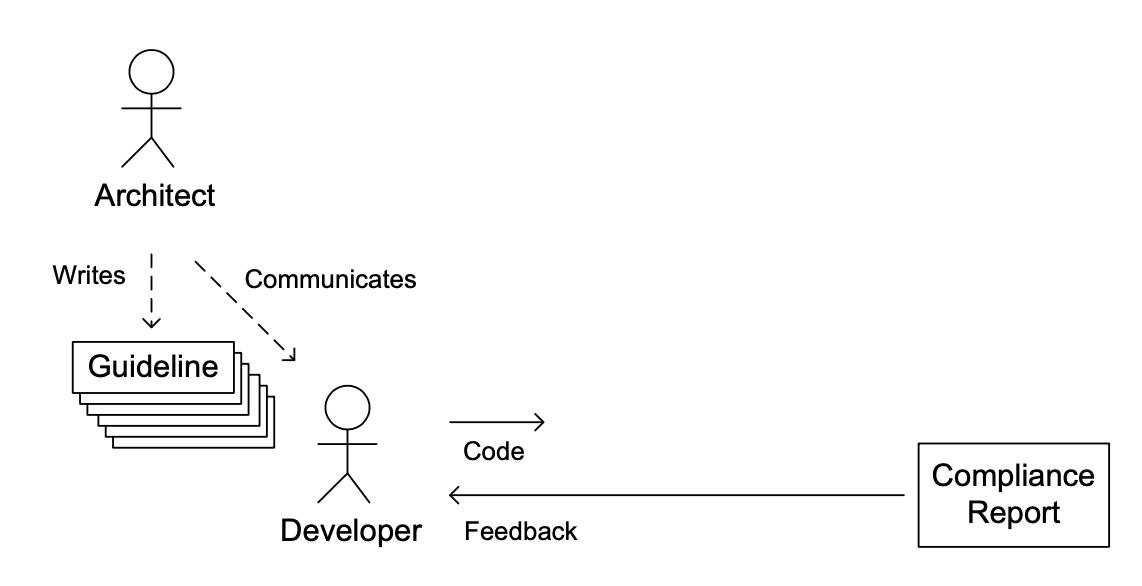
\includegraphics[width=0.7\textwidth]{../images/topic_9_approach_2_1.png}
	\caption{The common way of communicating architectural requirements~\cite{Lagerstedt2014}}
	\label{fig:topic_9_approach_2_1}
\end{figure}

This way of communicating guidelines is not very cost-efficient.
Every developer has to read and understand the guidelines. Developers must be re-trained when changes are made or if too many guidelines violations occur, because they have been forgotten.
This is quite time consuming and prone to error.  Creating reports about guideline compliance is time consuming as well.
Furthermore, while code review should be performed for all code changes, mistakes may slip through.

That is why the author proposes automated testing of software architecture \glspl{NFR}.
This allows a fast tool-based feedback loop in which the developer gets a code review that can be incorporated without other developers having to look out for violations of guidelines.
On top of that, by having this tight feedback loop, developers can learn the guidelines in an iterative way.
Little to no training is required, which saves time to make new guidelines known to all developers.

The guidelines are written as tests. These tests can be included in existing static code analysis tools such as linters and other code checkers. Developers can see the results of such tools.
Furthermore guidelines are communicated to the developer in case of a test failure.
Lagerstedt uses \autoref{fig:topic_9_approach_2_2} to visualize this approach.
Developers get feedback through different tools that the architect extends. Tools such as the editor, compiler or static analysis tools.

\begin{figure}[htbp]
	\centering
	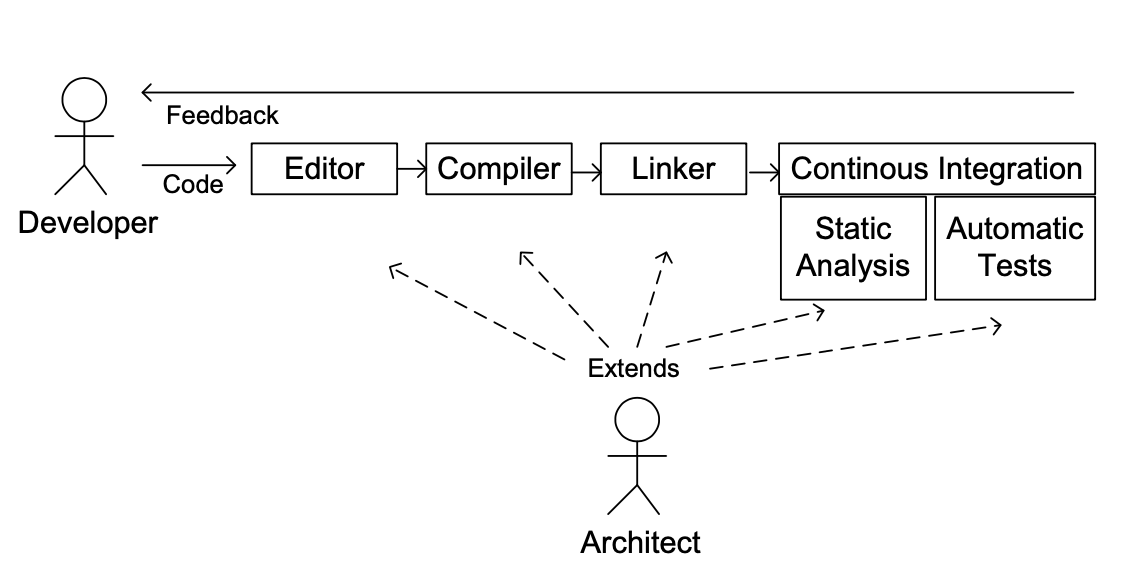
\includegraphics[width=0.7\textwidth]{../images/topic_9_approach_2_2.png}
	\caption{Suggested solution of communicating requirements~\cite{Lagerstedt2014}}
	\label{fig:topic_9_approach_2_2}
\end{figure}

According to Lagerstedt's personal experience, a tool based approach is superior to a guideline-only one.
Productivity is increased while the time spent on communicating architectural guidelines is decreased.
The number of non-compliant code is lower for the tool-based approach than for using guidelines and reports only.


\subsection{Application of Approach 2}

The paper works with architectural \glspl{NFR} but does not explain how those can be modeled.
To be able to apply the approach, we introduce another system function to the movie manager example that is listed in \autoref{tbl:topic_9_application_approach_2}.
This system function and the following \glspl{NFR} are based on personal experience in maintaining an open-source media manager.

\begin{table}[h!]
	\centering
	\caption{New system function for application of approach 2 of topic 9}
	\label{tbl:topic_9_application_approach_2}
	\begin{tabular}{rp{0.7\textwidth}}
		\textbf{Name}          & Export the movie to HTML \\
		\textbf{Description}   & An existing movie is exported to a single HTML file which can be viewed in any modern web browser \\
		\textbf{Precondition}  & Movie exists \\
		\textbf{Input}         & Movie details \\
		\textbf{Postcondition} & HTML file exists with the movie's contents \\
		\textbf{Output}        & HTML file \\
	\end{tabular}
\end{table}

In \autoref{tbl:topic_9_approach_2_nfr} on \autopageref{tbl:topic_9_approach_2_nfr}, two \glspl{NFR} are listed which were created for the system function in \autoref{tbl:topic_9_application_approach_2}. 
These two \glspl{NFR} are based on personal experience.
Both are transformed into pseudo code so that the \glspl{NFR} can be executed automatically as part of the code review.

While these two \glspl{NFR} can be written as guidelines, especially point two may be violated and may slip through code review. Violating point two may result in security issues or at least in unexpected behavior if the HTML contains unescaped characters.

\begin{longtable}[th]{p{0.05\textwidth}|p{0.24\textwidth}|p{0.65\textwidth}}
	\caption{\glspl{NFR} for the application of approach 2 of topic 9}
	\label{tbl:topic_9_approach_2_nfr}
	\setlength{\tabcolsep}{1em} \\    %%%%<===
	\textbf{No.} & \textbf{NFR} & \textbf{Explanation} \\
	\toprule
	1 & IMDb IDs are encapsulated in a class &
	All IMDb IDs have a certain format. They start with the string \enquote{tt} and end with 7-8 numbers. The ID must be validated which cannot be ensured by using a simple string. This is why an encapsulation in a class is required.
	
	Furthermore the programming language's type system can help to identify conversion bugs as well.
	\newline \newline \textit{Implementation in pseudo code}
	\begin{lstlisting}
for each $variable in $source:
 if $variable.startsWith("imdb") then
  if typeof($variable) != "ImdbId" then
   throw new Exception("Wrong class")
	\end{lstlisting}\\
	\midrule
	
	2 & Exported strings are escaped &
	This is a security concern and can be implemented in different ways. We assume that an HTML-exporter was created which takes a movie object as an argument.
	This object may contain texts which contain HTML elements themselves.
	These elements need to be escaped. To ensure this \glspl{NFR}, all strings must be run through a certain function which escapes strings.
	
	Because this may be missed by the developer, a new string-subclass is introduced which escapes its input automatically, e.g. \texttt{EscapedString}.
	Only this string class may be used in the HTML exporter.
	\newline \newline \textit{Implementation in pseudo code}
	
	\begin{lstlisting}
for each $functionCall in $HTMLExporter:
 if $functionCall == "writeText" then
  $arg = argument of($functionCall);
  if typeof($arg) != "EscapedString" then
   throw new Exception("Wrong class")
	\end{lstlisting}

\textit{Note:} We assume that \texttt{writeText} is a method of a generic HTML-class which the HTML-exporter uses itself. We assume that the method cannot be changed to accept another argument type. Otherwise the language's type checker could already be able to find this issue.\\

\bottomrule
\end{longtable}


%%%%%%%%%%%%%%%%%%%%%%%%%%%%%%%%%%%%%%%%%%%%%%%%%%%%%%%%%%%%%%%%%%%%%%%%%%%%%%
%%%%%%%%%%%%%%%%%%%%%%%%%%%%%%%%%%%%%%%%%%%%%%%%%%%%%%%%%%%%%%%%%%%%%%%%%%%%%%
\clearpage
\section{Comparison} \label{sec:9_comparison}

For an improved comparison of these two approaches, a synthesis matrix is provided which references the following questions:

\begin{enumerate}
	\item Description of the approach (What does the approach do?)
	\begin{enumerate}
		\item Which artifacts and relations between artifacts are used in this approach? Which artifacts are created in the course of the approach? How are the artifacts characterized?
		\item What is required and/or input for the application of the approach?
		\item Which steps does the approach consist of? Which information is used in which step and how? What are the results of the individual steps?
	\end{enumerate}
	\item Benefits of the approach (Whom does the approach help and how?)
	\begin{enumerate}
		\item Which usage scenarios are supported by the approach?
		\item Which stakeholders are supported by the usage scenarios?
		\item Which knowledge areas from SWEBOK can be assigned to the usage scenarios?
	\end{enumerate}
	\item Tool support for the approach (What tool support is available?)
	\begin{enumerate}
		\item What kind of tool support is provided for the approach?
		\item Which steps of the approach are automated by a tool? Which steps are supported by a tool, but still have to be executed manually? Which steps are not supported by a tool?
	\end{enumerate}
	\item Quality of the approach (How well does the approach work?)
	\begin{enumerate}
		\item How was the approach evaluated?
		\item What are the (main) results of the evaluation?
	\end{enumerate}
\end{enumerate}


\begin{longtable}[h]{p{0.02\linewidth}p{0.45\linewidth}p{0.45\linewidth}}
	\centering
	\textbf{No.} & \textbf{Approach 1 \cite{ZouPavlovski2008}} & \textbf{Approach 2 \cite{Lagerstedt2014}} \\
	\textbf{1a} & 
	Operating conditions are formed that work under specific use cases.
	These, on the other, hand are controlled by control cases and can be operated under them.
	Control cases describe the business risks in case that the operating condition cannot be fulfilled.
	Because use cases and control cases are tightly connected to each other, they can be modeled in one consolidated model.
	& 
	
	Coding guidelines are written and transformed into tests that can be used by tools in code review.
	These point out issues that the developer can fix.
	Guidelines are characterized by the fact that they describe the code architecture.
	\\
	
	\textbf{1b} & 
	There are no preconditions because we start defining control cases at the beginning of the software development process, for example at the \enquote{Business Process Modelling}-step.
	
	&
	The guidelines cover code architecture. They must be transformable into automated tests (e.g. by a static code analyzer).
	
	\\
	
	\textbf{1c} &
	Preconditions/Constraints must be extracted from which \glspl{NFR} are created, e.g. performance or security constraints.
	These constraints are modeled by operating conditions for which control cases are created.
	Their purpose is to mitigate business risk which is essentially the failure to fulfill the operating condition.
	For each control case a test case is added that checks if the controls put in place by the control case are effective.
	The test case basically recreates the operating condition, for example by using stress testing.
	
	&
	Code guidelines such as naming conventions or prohibited function-calls are defined.
	These are transformed into automated tests that can be executed by the developer (i.e. a tool based approach).
	The exact process is not explained and it is left to the reader how this may be implemented.
	It is only pointed out that existing tools such as compilers or static code analysis tools can be extended and used.
	\\
	
	\textbf{2a} & 
	
	Early modeling of non-functional requirements. Being able to control requirements throughout the whole software development life cycle.
	
	&
	Maintainability, quality and security of the code base can be hold up to standards and may even be improved by giving automated feedback that points out \glspl{NFR} which are violated by the developer.
	
	\\
	
	\textbf{2b} & 
	Management, Requirements Engineer, Developers, Testers
	&
	Developer / test writer, Software Architect
	\\
	
	\textbf{2c} &
	Software Requirements (functional and non-functional requirements, acceptance tests), Software Testing (model based techniques)
	&
	Software Testing (Software Testing Tools, Test Techniques), Software Maintenance (Software Maintenance Tools) \\
	
	\textbf{3a} & 
	No tool support for generating \enquote{Control Case}-Boxes and other artifacts &
	Existing static code analysis tools (e.g. linters), which can be extended by further tests.
	\\
	\textbf{3b} & 
	No automation is done. Automation is only proposed as another step which can be implemented, e.g. through code generation with SysML.
	&
	Only code testing is performed automatically.
	And only tests for \glspl{NFR} which were extracted from the software architects guidelines and that were transformed into automated tests.
	Those tests can be executed automatically during code review, e.g. by a continuous-integration service which tests each code change. Writing the tests is still a manual job.
	\\
	
	\textbf{4a} 	
	&
	The approach was explained by creating a fictional example and going through all steps of the software development life cycle by extending the example. No evaluation was performed, though.
	
	&
	No evaluation was performed. The conclusion, i.e. success of the approach, is based on personal experience only.
	\\
	
	\textbf{4b} &
	N/A &
	
	Based on his experience in both small and large organizations, Lagerstedt concludes that automated verification of non-functional requirements by using tool-chain feedback is superior to classic guidelines that need to be checked by humans. By evaluation of his prior experience, he concludes increased productivity and a decrease in time spent on communicating architectural requirements. \\
\end{longtable}


If we compare the two papers using the synthesis matrix above, we notice that they do not share a lot.
That is not surprising: the second paper is very specific and only deals with architectural \glspl{NFR} in code.
The first paper, on the other hand, can be applied to different \glspl{NFR}, not limiting itself to a specific one.
Only the first paper mentions risk analysis but only as part of a control case.

Both papers do not give specific instructions how test cases can be modeled.
While the first paper only says to \enquote{simulate the operating condition}~\cite{ZouPavlovski2008}, it leaves out details.
For example security \glspl{NFR} are explicitly mentioned but it is left out how an operating condition for that \gls{NFR} can be simulated.
Also the example test case from the paper is essentially a stress test.
The second paper leaves it to the reader to develop automated tests and only mentions that static code analysis tools can be used.

While the second paper talks about test automation, it does not talk about creating tests automatically but rather about running them automatically~\citealp{Lagerstedt2014}.
The first paper does not include any automation step at all.
Neither for creating test cases automatically nor for running them.

Both do not include an evaluation of their results besides personal experience.
The first article states no evaluation at all and only discusses the approach for defining the control case.


%%%%%%%%%%%%%%%%%%%%%%%%%%%%%%%%%%%%%%%%%%%%%%%%%%%%%%%%%%%%%%%%%%%%%%%%%%%%%%
%%%%%%%%%%%%%%%%%%%%%%%%%%%%%%%%%%%%%%%%%%%%%%%%%%%%%%%%%%%%%%%%%%%%%%%%%%%%%%

\section{Conclusion} \label{sec:9_conclusion}

Both articles deal with \glspl{NFR}.
While \cite{ZouPavlovski2008} describes how these can be defined and controlled, it does not specify a way to test them except for simulating the operating condition.
In the same way there is no description of how the business risk affects the test case except for defining the test-priority.
However, it explains in great detail how control cases and operating conditions can be defined and how they interact with use cases and functional requirements, which raised my interest in the overall topic of testing \glspl{NFR}.
But the lack of detailed explanation for test case creation makes it difficult for me to assess the usefulness of the approach. After reading the paper I may know how to model \glspl{NFR} with operating conditions but still wonder how they can be properly tested.

\cite{Lagerstedt2014} on the other hand leaves it to software architects to define \glspl{NFR}.
The paper only uses architectural \glspl{NFR} that exist as code conventions and other guidelines.
The author describes why having automated tests is a necessity of software development in regards to cost efficiency and how it mitigates human error during code review which can be seen as a risk to code maintainability.
This corresponds to my personal experience. 
By using a code formatter, the amount of formatting related review comments went down to zero.
By introducing a new linter rule, I was able to automatically fix company branding issues in product messages which none of my colleagues were even aware of.
I can therefore only emphasize that communication of \glspl{NFR} is more effective and  efficient when a tool based approach is used.


Finally, both articles mention risk analysis only as a side note, if mentioned at all.
It is left to the reader where risks are mitigated.
The conclusion is that \glspl{NFR} with higher risks need to be paid more attention to by giving the tests higher priority.

